
\section{Methodology}
\label{section:methodology}

\begin{figure}[H]
  \hspace{-20mm}
    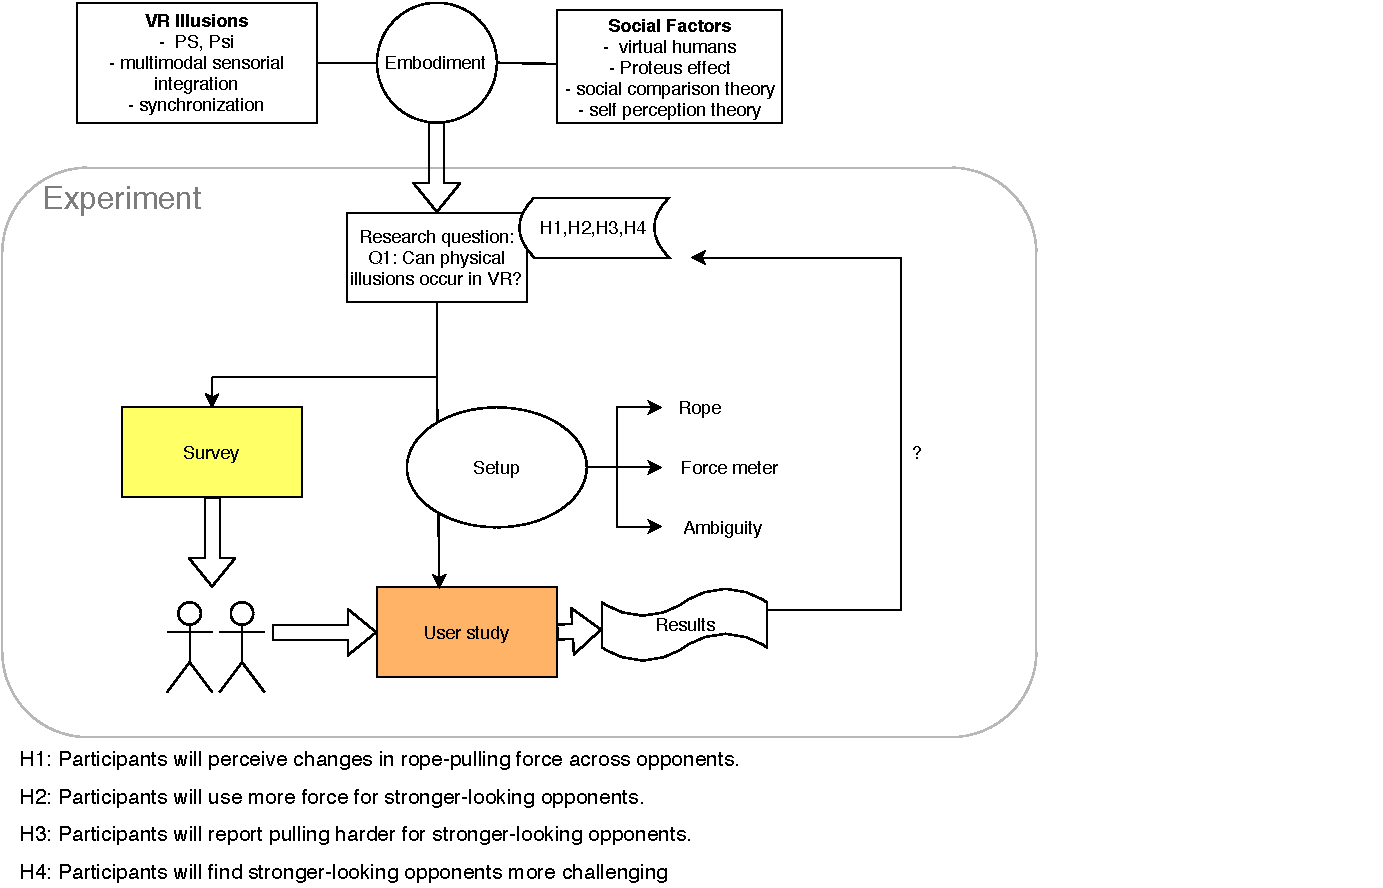
\includegraphics[scale=1]{Files/diagram.pdf}
    \caption{Methodology overview.}
     \label{fig:SurveyRatedMmalesAll}
    \end{figure}

\clearpage
The experiment has two parts: a survey and a user study. We run a survey in order to determine perceptions of strength and intimidation in avatar design. We measure perceived strength and intimidation for avatars and vary the appearance based on a weighted score of these two measures. We choose the avatars for the experiment based on the survey results. Please see section \ref{section:survey} for more details about the survey and choice of avatars.
\subsection{Research Aims}
The aim of our experiment is two-fold. Firstly we explore the feasibility of generating physical illusions in virtual reality (\textbf{Q1}).To do this, we implement a VR tug-of-war game and vary the appearance of participants' opponents. Our independent variable is the appearance of the opponent. Each opponent will randomly be assigned a condition of this variable, from weak-looking to strong-looking. We determine the appearance perception in a survey (see \ref{section:surveyResults}) and the number of conditions through piloting (see \ref{subsection:Piloting}).  We investigate if participants perceive any change in rope-pulling from one trial to another. We formalize our first hypothesis:
\begin{quote}
\textbf{H1}: \textit{Participants will perceive changes in rope-pulling force across opponents.}
\end{quote}
To measure any perceived changes in rope pull, we introduce a dependent variable, \textbf{challenge}. We ask participants to rate how challenging each rope-pull was after the respective trial. We do not give any indication for a standard to be applied for this rating. We leave it to the participant to interpret what \textit{challenging} means.\\ Additionally, we introduce \textbf{perceived pull} as a subjective measure of how much participants thought they pulled. We measure both variables on a 5-point Likeart scale. For each condition, we also take objective measurements of actual pull. We use a force meter to detect the maximum force each participant pulled per trial. This constitutes the the third dependent variable, \textbf{force}. We expect users to react to the appearance of their opponent and pull harder for stronger-looking opponents. We formalize the hypotheses of these variables:\\

\textbf{H2}: \textit{Participants will use more force for stronger-looking opponents.}\\

\textbf{H3}: \textit{Participants will report pulling harder for stronger-looking opponents.}\\

\textbf{H4:}\textit{ Participants will find stronger-looking opponents more challenging.}\\
\\
For H2, we use the maximum pull per trial as a measure of \textit{more force}. 
We do not make it explicit that participants are competing with an agent. We set up the rope pulling game in an ambiguous manner, such that participants do not see the pulling mechanism. Ultimately, we are interested in the feasibility of generating very implausible illusions in VR. Giving the impression that another human player is pulling the rope is one example of such an illusion that can be generated with this setup. 

\subsection{Study Design}
To investigate the actual variation in force determined by the avatars, we run a user study in which participants play a tug-of-war game. The study has a within-subjects design varying the appearance of the opponent avatar in terms of strength and intimidation. We use a 5 point scale from weak to strong-looking. Our independent variable is the appearance of the opponent's avatar. We have 3 additional dependent variables, challenge, pull and force. Through mixed methods, we also measure presence in the virtual environment, co-presence with the opponents and body ownership of the participant. This design reflects the holistic approach of our research methods. We endeavour to collect quantitative objective data, subjective experiences and qualitative feedback. We believe this approach is necessary to accurately and consistently frame of our results. Having multiple perspectives allows for at least a minimal validation of our conclusions. We hope that our data will be mirrored in participants' feedback. Furthermore, qualitative data can be used to explain unexpected quantitative variations.
\\
We frame our research in the context of a competitive strength task between a user and a perceived agent in virtual reality. A competitive set up allows participants to face their opponents directly in a physical task. Furthermore, it constitutes a realistic interaction for a game setup.  Players are told they are testing a rope pulling VR game and they are be asked for feedback and suggestions to improve the game.
Their task is to face several different \textit{opponents} in VR, compete at pulling a rope and win. The player is able to see their hands in the virtual environment holding the rope. They are instructed to keep their hands on the rope at all times. Since their fingers are not animated and the grip is fixed on the rope, letting go of the rope might result in breaks of presence and ownership. We do not mention the nature of the opponent as we would like to investigate what assumptions participants have. We do not make the aim of our research transparent, to avoid any possible biases, such as the observer expectancy effect, or induce powerful demand characteristics.
\\
For the game, participants use VR gloves and hold a real, physical rope that corresponds to the virtual rope. Rope-pull time will be adjusted through piloting. The present set up is a low fidelity version of the user study. The opponents do not respond to participants' pull, and there is no force activating on the rope. We use a spring and an elastic band to give some resistance when participants pull. To maintain the appearance of realism, we use animations, game physics and sound.\\
We pay particular attention to timing and synchronization in the design of the game. As noted in \cite{kilteni2012sense}, congruence between visuomotor actions gives rise to agency and ownership is determined by synchronized haptic and/or visual feedback. We combine and leverage these synchronicities to match the expected outcome of peoples actions. Such \textit{sorimotor contingencies} \cite{slater2009place} allows us to create a context viable for giving rise to VR physical illusions. We use spring resistance to give participants some motor sensations. After all, the rope moving towards them is something they expect to happen in a rope-pulling game. Realistic interactions that allow visual and sensorial synchronization seem to contribute to the formation of these illusions \cite{slater2009place}. The ambiguous source of the motor feedback and its magnitude is what participants will have to discern.
\\
Participants see a countdown accompanied by sounds for each visual element being displayed. They are told to start pulling when they see \textit{start}, and stop pulling when they see \textit{stop}. When participants start pulling, they also see their opponent pulling and feel the resistance increase on the rope as they go on. Through this flow of events we synchronize, visual, audio and haptic feedback in order to give users the impression of agency and realism. With this low fidelity set up, we explore whether participants perceived any changes in the rope pull. In a high fidelity set up, we would use motors to pull the rope to generate the illusion that another human player is pulling. 